\section{The Bailout Protocol}
\label{sec:bailout}

\subsection{Overview and Motivation}
The Bailout Protocol is a deterministic vertical-escalation mechanism within the BX3 Framework's Fact Layer. It provides a guaranteed escape path when the Truth Gate rejects an action, when an agent cannot autonomously resolve a constraint conflict, or when the system's bounded autonomy boundary has been reached. Unlike the Training Wheels Protocol, which governs the system's general mode of operation, the Bailout Protocol is event-driven: it activates in response to specific failure conditions and bypasses all machine actors to route accountability to a designated human resolver.

The protocol defines a finite state machine with six states, formal transition predicates, a bail-out trigger condition, an escalation algorithm with timeout handling, and a bypass mechanism that renders all machine-level actors moot once a bailout is initiated.

\subsection{State Machine Definition}
\label{sec:states}

The protocol state space is defined as a 6-tuple:

\begin{equation}
\mathcal{S} = \{ \text{IDLE}, \text{BOUNDED}, \text{BAIL\_PENDING}, \text{ESCALATING}, \text{HUMAN\_ACKNOWLEDGED}, \text{RESOLVED} \}
\end{equation}

Each state encodes a distinct phase of the escalation lifecycle.

\medskip\noindent\textbf{IDLE.} The system is operating normally. No escalation conditions are active. All agent actions proceed through the Truth Gate and Bounds Engine without triggering.

\medskip\noindent\textbf{BOUNDED.} The system has detected a condition that places it at the boundary of its operational autonomy. This is not yet a failure --- the system is still processing within its bounds, but a structural constraint is under tension. Examples: an action's risk score is within 5\% of the bounds threshold; a sensor reading is approaching a defined safety limit; a time budget is within one standard deviation of depletion.

\medskip\noindent\textbf{BAIL\_PENDING.} A bail-out trigger condition (Section~\ref{sec:trigger}) has fired. The action or condition has been logged and is awaiting formal escalation. No human contact has been initiated.

\medskip\noindent\textbf{ESCALATING.} The escalation algorithm (Section~\ref{sec:escalation}) has been invoked. All machine actors are suspended for the duration of this state. The human resolver is being notified through all configured channels.

\medskip\noindent\textbf{HUMAN\_ACKNOWLEDGED.} A human resolver has received the escalation and has acknowledged it. The machine actors remain suspended. The human now has the decision authority that the system could not autonomously resolve.

\medskip\noindent\textbf{RESOLVED.} The human resolver has issued a decision. The decision is logged to the forensic ledger. The system transitions to IDLE, and all machine actors resume.

\begin{figure}[H]
\centering
\begin{tikzpicture}[node distance=2.8cm, semithick, >=stealth]
  \node[state] (IDLE) {$IDLE$};
  \node[state, right of=IDLE] (BOUNDED) {$BOUNDED$};
  \node[state, right of=BOUNDED] (BAIL\_PENDING) {$BAIL\_PENDING$};
  \node[state, below of=BAIL\_PENDING] (ESCALATING) {$ESCALATING$};
  \node[state, left of=ESCALATING] (HUMAN\_ACK) {$HUMAN\_ACKNOWLEDGED$};
  \node[state, left of=HUMAN\_ACK] (RESOLVED) {$RESOLVED$};

  \draw (IDLE) edge[->] node[above] {$boundary\_condition$} (BOUNDED);
  \draw (BOUNDED) edge[->] node[above] {$trigger\_condition$} (BAIL\_PENDING);
  \draw (BAIL\_PENDING) edge[->] node[right] {$escalate\_now$} (ESCALATING);
  \draw (ESCALATING) edge[->] node[above] {$human\_ack$} (HUMAN\_ACK);
  \draw (HUMAN\_ACK) edge[->] node[above] {$decision\_logged$} (RESOLVED);
  \draw (RESOLVED) edge[->, bend left=20] node[below] {$reset$} (IDLE);
  \draw (BAIL\_PENDING) edge[->, bend left=15] node[left] {$timeout$} (ESCALATING);
  \draw (HUMAN\_ACK) edge[->, bend right=15] node[below] {$human\_timeout$} (ESCALATING);
\end{tikzpicture}
\caption{Bailout Protocol State Machine}
\label{fig:state-machine}
\end{figure}

\subsection{Transition Conditions}
\label{sec:transitions}

Each state transition is gated by a formal predicate. Transitions are atomic and deterministic: if the predicate evaluates to true, the transition fires; otherwise, the system remains in the current state.

\begin{table}[H]
\centering
\caption{State Transition Table}
\label{tab:transitions}
\begin{tabular}{@{}lp{5.5cm}l@{}}
\toprule
\textbf{From} & \textbf{Predicate (Condition)} & \textbf{To} \\
\midrule
IDLE & $boundary\_condition()$ evaluates true & BOUNDED \\
BOUNDED & $trigger\_condition()$ evaluates true & BAIL\_PENDING \\
BOUNDED & $boundary\_condition()$ clears without trigger & IDLE \\
BAIL\_PENDING & $escalate\_now()$ is called & ESCALATING \\
BAIL\_PENDING & $t_{elapsed} > T_{escalate}$ (timeout) & ESCALATING \\
ESCALATING & Human acknowledges via any channel & HUMAN\_ACKNOWLEDGED \\
HUMAN\_ACKNOWLEDGED & Decision logged to forensic ledger & RESOLVED \\
HUMAN\_ACKNOWLEDGED & $t_{elapsed} > T_{human}$ (human timeout) & ESCALATING \\
RESOLVED & $reset()$ called after post-processing & IDLE \\
\bottomrule
\end{tabular}
\end{table}

The predicates are defined as follows:

\begin{itemize}
  \item $boundary\_condition() \equiv \exists\, a \in Actions : risk(a) \geq \theta_{bounded} \land risk(a) < \theta_{trigger}$
  \item $trigger\_condition() \equiv \exists\, a \in Actions : risk(a) \geq \theta_{trigger} \lor truth\_gate(a) = \perp \lor bounded\_actor(a) = \bot$
  \item $human\_ack() \equiv \exists\, h \in HumanResolvers : ack\_received(h, escalation\_id) = \top$
  \item $decision\_logged() \equiv forensic\_ledger.append(decision\_record) = \top$
\end{itemize}

The thresholds $\theta_{bounded}$ and $\theta_{trigger}$ are set by the Purpose Layer and satisfy $0 < \theta_{bounded} < \theta_{trigger} \leq 1$.

\subsection{Bail-Out Trigger Condition}
\label{sec:trigger}

The bail-out trigger condition is the canonical event that advances the system from BOUNDED to BAIL\_PENDING. It fires when any one of three mutually non-exclusive conditions is true:

\begin{equation}
trigger\_condition() \triangleq
\begin{cases}
\text{Risk Threshold:} & \exists\, a \in Actions : risk(a) \geq \theta_{trigger} \\[4pt]
\text{Truth Gate Failure:} & \exists\, a \in Actions : truth\_gate(a) = \perp \\[4pt]
\text{Autonomy Boundary:} & \exists\, a \in Actions : bounded\_actor(a) = \bot
\end{cases}
\end{equation}

\medskip\noindent\textbf{Risk Threshold.} The action's computed risk score exceeds $\theta_{trigger}$. This covers high-consequence actions (financial transactions above a configurable ceiling, public-facing communications, data deletions, or safety-critical actuator commands).

\medskip\noindent\textbf{Truth Gate Failure.} The Truth Gate (Section~4 of the BX3 Framework paper) returns $\perp$ (undefined/rejected) for the action. This is the canonical alignment failure signal. When $truth\_gate(a) = \perp$, the action cannot proceed through any machine actor --- the chain of trust is broken.

\medskip\noindent\textbf{Autonomy Boundary.} The action requires a capability or authorization level that no registered bounded actor possesses. This occurs when the task decomposition chain produces an action that was not anticipated in the system's original capability bounds. The action is structurally within the system but operationally outside the competence envelope.

When any trigger condition fires, the Fact Layer atomically: (1) records the trigger event to the forensic ledger with full context; (2) transitions the escalation state machine to BAIL\_PENDING; and (3) suspends the originating agent from further action on the affected task.

\subsection{Escalation Algorithm}
\label{sec:escalation}

The escalation algorithm governs the ESCALATING state. It is invoked immediately upon transition from BAIL\_PENDING (either via $escalate\_now()$ or upon timeout expiration).

\begin{algorithm}
\caption{Bailout Escalation Algorithm}
\label{alg:escalation}
\begin{enumerate}
  \item \textbf{Suspend all machine actors.} Set $actor.suspended \leftarrow \top$ for all $actor \in MachineActors$. No agent may take action on the affected task during ESCALATING. This is architecturally enforced in the Fact Layer --- no code path bypasses this step.

  \item \textbf{Construct escalation record.} Assemble $E = \{escalation\_id, timestamp, trigger\_condition, affected\_task, affected\_actor, context\_snapshot, risk\_score, human\_channels\}$.

  \item \textbf{Notify human resolvers.} For each channel $c \in human\_channels$, dispatch notification:
  \begin{itemize}
    \itemsep0em
    \item SMS to primary resolver (guaranteed delivery, $T_{sms} < 30$s)
    \item Email to primary and secondary resolver queues
    \item Push notification via connected device channels
    \item Discord DM if configured
  \end{itemize}

  \item \textbf{Start human timeout timer.} Set $T_{human\_timer} \leftarrow now()$. If no acknowledgement is received within $T_{human}$ seconds, re-notify and increment escalation level.

  \item \textbf{Await acknowledgement.} Block machine actors. Return control to event loop. Transition to HUMAN\_ACKNOWLEDGED upon $human\_ack()$.

  \item \textbf{On timeout before acknowledgement:} Re-dispatch notifications to all channels. Increment escalation priority. Log $timeout\_event$ to forensic ledger. Remain in ESCALATING.
\end{enumerate}
\end{algorithm}

The escalation record $E$ is the single source of truth for the human resolver. It contains the full action context, including: the exact prompt or action that triggered the bailout, the Truth Gate output or constraint that caused the failure, the complete intent chain from the root task to the triggering action, and all relevant sensor data or external inputs at the time of trigger.

\subsection{Bypass Mechanism}
\label{sec:bypass}

The bypass mechanism is the architectural guarantee that the Bailout Protocol, once activated, overrides all machine actors without exception. This is a structural property, not a policy setting.

\begin{figure}[H]
\centering
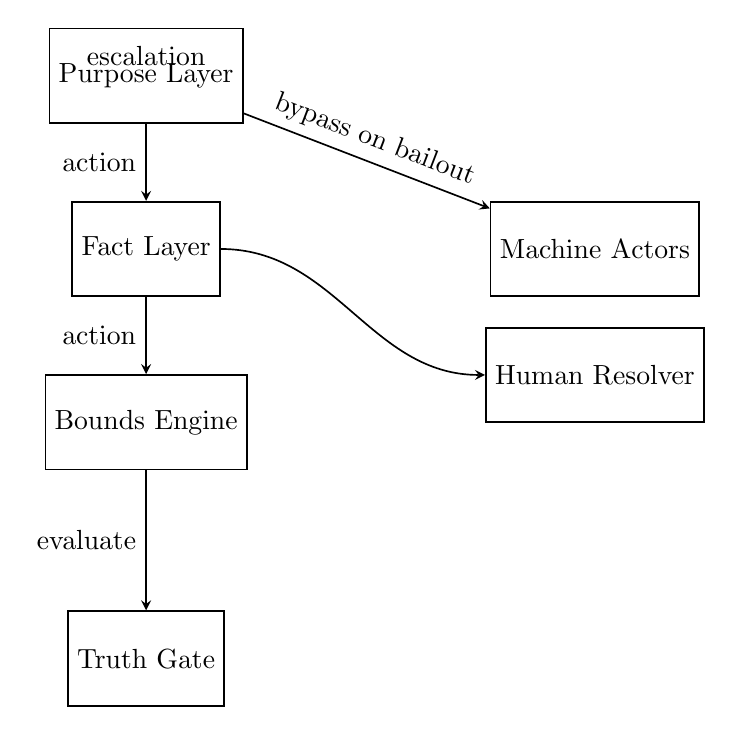
\begin{tikzpicture}[node distance=2.2cm, semithick, >=stealth]
  \node[draw, rectangle, minimum height=1.2cm] (PL) {Purpose Layer};
  \node[draw, rectangle, minimum height=1.2cm, below of=PL] (FL) {Fact Layer};
  \node[draw, rectangle, minimum height=1.2cm, below of=FL] (BE) {Bounds Engine};
  \node[draw, rectangle, minimum height=1.2cm, below of=BE, yshift=-0.8cm] (TG) {Truth Gate};

  \node[draw, rectangle, minimum height=1.2cm, right of=FL, xshift=3.5cm] (MA) {Machine Actors};
  \node[draw, rectangle, minimum height=1.2cm, right of=FL, xshift=3.5cm, yshift=-1.6cm] (HR) {Human Resolver};

  \draw[->] (PL) -- (FL) node[midway, left] {action};
  \draw[->] (FL) -- (BE) node[midway, left] {action};
  \draw[->] (BE) -- (TG) node[midway, left] {evaluate};
  \draw[->] (PL) -- (MA) node[midway, above, sloped] {bypass on bailout};
  \draw[->] (FL) to[out=0, in=180] (HR) node[midway, above] {escalation};
\end{tikzpicture}
\caption{Bypass Path: Direct Fact Layer $\rightarrow$ Human Resolver}
\label{fig:bypass}
\end{figure}

During normal operation, an action flows: Purpose Layer $\rightarrow$ Bounds Engine $\rightarrow$ Truth Gate $\rightarrow$ Machine Actor $\rightarrow$ execution. When the bail-out trigger condition fires, the Fact Layer severs this path and redirects control directly to the Human Resolver, bypassing the Purpose Layer, Bounds Engine, Truth Gate, and all Machine Actors.

The bypass is implemented as a hard interrupt in the Fact Layer:

\begin{verbatim}
function process_action(action a):
    if bailout_state == IDLE or bailout_state == BOUNDED:
        proceed through normal pipeline
    elif bailout_state in {BAIL_PENDING, ESCALATING,
                          HUMAN_ACKNOWLEDGED, RESOLVED}:
        # Bypass all machine actors
        escalate_to_human(a, context_snapshot)
        suspend(a.originator)
        return  # no further machine processing
\end{verbatim}

Because the Fact Layer is architecturally isolated from the Purpose Layer and Bounds Engine, no machine actor can override or suppress a bailout once the Fact Layer has initiated escalation. This is not a privilege level --- it is a structural cut in the execution graph. Even a fully compromised Purpose Layer cannot re-route a bailout in progress.

This property is what makes the Bailout Protocol trustworthy as a last resort. The human resolver is the only actor with decision authority during a bailout, and this authority is architecturally guaranteed.

\subsection{Timeout Handling}
\label{sec:timeouts}

The protocol defines two timeout windows:

\begin{table}[H]
\centering
\caption{Bailout Timeout Parameters}
\label{tab:timeouts}
\begin{tabular}{@{}lp{3cm}l@{}}
\toprule
\textbf{Timeout} & \textbf{Default Value} & \textbf{Governs} \\
\midrule
$T_{escalate}$ & 60 seconds & IDLE $\rightarrow$ BAIL\_PENDING $\rightarrow$ ESCALATING \\
$T_{human}$    & 300 seconds & ESCALATING $\rightarrow$ HUMAN\_ACKNOWLEDGED \\
\bottomrule
\end{tabular}
\end{table}

\medskip\noindent\textbf{Escalation Timeout ($T_{escalate}$).} Once in BAIL\_PENDING, if the system does not call $escalate\_now()$ within $T_{escalate}$ seconds, the state machine automatically transitions to ESCALATING. This prevents BAIL\_PENDING from becoming a dead state if a bounded actor fails to invoke escalation due to a software fault. $T_{escalate}$ is measured by the Fact Layer's internal clock, not by any agent.

\medskip\noindent\textbf{Human Timeout ($T_{human}$).} Once in ESCALATING, if no human acknowledgement is received within $T_{human}$ seconds, the protocol re-dispatches notifications at higher priority (all channels simultaneously) and logs the timeout event to the forensic ledger. After $2 \times T_{human}$ without acknowledgement, the protocol enters a sustained alert state: the system remains suspended, all designated resolvers are notified via out-of-band channels (SMS repeat, escalation email), and a P1 alert is logged to INBOX.md for brodiblanco. The system does not automatically resume operation --- a human must explicitly acknowledge and resolve.

\medskip\noindent\textbf{Timeout Override.} The Purpose Layer may increase or decrease timeout values based on task criticality. Time-sensitive tasks (e.g., irrigation actuator decisions in Irrig8) have shorter timeouts; strategic tasks may have longer ones. The timeout override is set at task creation time and is immutable for the duration of the task.

\medskip\noindent\textbf{Clock Independence.} Timeout timers are maintained by the Fact Layer's independent clock, not by any agent process. This prevents clock manipulation by a compromised agent from suppressing timeouts.

\subsection{Formal Properties}
\label{sec:properties}

The Bailout Protocol satisfies three formal properties:

\medskip\noindent\textbf{Property 1 (Bypass Soundness).} If the bail-out trigger condition fires, the Human Resolver will receive the escalation before any machine actor takes action on the affected task.

\textit{Proof.} The trigger condition atomically (a) suspends the originating agent, (b) severs the action pipeline in the Fact Layer, and (c) initiates $escalate\_to\_human()$. Steps (a)--(c) are executed in the Fact Layer before any continuation of the agent event loop. The human notification is dispatched concurrently. By the time any agent could resume action on the affected task, the escalation is in ESCALATING state and $actor.suspended = \top$ for all machine actors. $\square$

\medskip\noindent\textbf{Property 2 (No Suppression).} No machine actor, including the Purpose Layer, can suppress, override, or delay a bailout once the trigger condition has fired.

\textit{Proof.} The trigger condition is evaluated and enforced in the Fact Layer. The Fact Layer has no upstream dependency on the Purpose Layer for enforcement. The Purpose Layer cannot modify $actor.suspended$ flags. The $escalate\_to\_human()$ call is unconditional upon trigger evaluation. $\square$

\medskip\noindent\textbf{Property 3 (Deterministic Resolution).} The system cannot transition from HUMAN\_ACKNOWLEDGED to RESOLVED without a logged decision from a human resolver.

\textit{Proof.} The transition $human\_ack \rightarrow RESOLVED$ requires $decision\_logged() = \top$, where $decision\_logged()$ returns true only if the forensic ledger append operation succeeds. The forensic ledger append requires a human-authored decision payload. No machine actor can fabricate a decision payload that passes the ledger's integrity check (SHA-256 sealed). $\square$

\subsection{Relationship to Training Wheels Protocol}
The Bailout Protocol operates orthogonally to the Training Wheels Protocol (Paper~\hyperref[sec16]{16}). The Training Wheels Protocol governs the system's general mode of operation (HITL Active, Shadow Mode, Full Autonomy, Lockdown) based on aggregate trust scores. The Bailout Protocol is event-driven and governs the escalation path within any training wheels mode. Even a system in Full Autonomy (Training Wheels Mode 0) is subject to the Bailout Protocol: if the Truth Gate fails or a high-risk trigger condition fires, the bailout path activates and suspends all machine actors, including those operating under full autonomy. The Training Wheels Protocol's Lockdown mode (Mode 3) is itself a terminal form of bailout, but the Bailout Protocol generalizes this concept to all escalation scenarios rather than restricting it to trust-score-driven mode transitions.

\end{document}
